%\documentclass[a4paper,12pt]{article}
\documentclass{amsart}
%\usepackage[utf8x]{inputenc}

\usepackage{amsmath}    % need for subequations
\usepackage{graphicx}   % need for figures
\usepackage{verbatim}   % useful for program listings
\usepackage{amssymb}
\usepackage{animate}
\usepackage{xcolor}
\usepackage{amsthm}
%\usepackage[margin=0.7in]{geometry}
\usepackage{mathrsfs}
\usepackage{bbm}
\usepackage{exscale}
\usepackage{enumerate}
\newtheorem{theorem}{Theorem}
\newtheorem{lemma}[theorem]{Lemma}
\newtheorem{corollary}[theorem]{Corollary}
\newtheorem{proposition}[theorem]{Proposition}
\newtheorem{problem}[theorem]{Problem}

\newtheorem{remark}[theorem]{Remark}

\theoremstyle{remark}
\newtheorem{rem}[theorem]{Remark}

\theoremstyle{definition}
\newtheorem{example}[theorem]{Example}
\newtheorem{definition}[theorem]{Definition}
%My Commands
\newcommand{\finsum}[3]{
\underset{#1=#2}{\overset{#3}\sum}}

\newcommand{\dint}{\displaystyle\int}
\newcommand{\dsum}{\displaystyle\sum}

\newcommand{\sgn}{\textnormal{sgn}}
\newcommand{\R}{\mathbb{R}}
\newcommand{\C}{\mathbb{C}}
\newcommand{\N}{\mathbb{N}}
\newcommand{\Z}{\mathbb{Z}}
\newcommand{\F}{\mathscr{F}}
\newcommand{\supp}{\textnormal{supp}}
\newcommand{\T}{\mathbb{T}}
\newcommand{\eps}{\varepsilon}


\newcommand{\ftilde}{\tilde{f}}
\newcommand{\sinc}{\textnormal{sinc}}
\newcommand{\schwartz}{\mathscr{S}}
\newcommand{\bracket}[1]{\left\langle#1\right\rangle}
\newcommand{\argmin}{\textnormal{argmin}}

 \newcommand{\floor}[1]{
 \lfloor#1\rfloor}
 \newcommand{\ceiling}[1]{
 \lceil#1\rceil}
 %End Commands

 \hyphenation{band-limit-ed}
\hyphenation{Band-limit-ed}
 
\title{Notes on Almost Isometries}
\author{Keaton Hamm}
\begin{document}
\maketitle

\section{Definitions}

\begin{definition}
Let $\eps>0$, and $\phi:\R^d\to\R^d$ be a diffeomorphism, and let $I$ be the $d\times d$ identity matrix.  Then we say that $\phi$ is $\eps$--\textit{distorted} provided the following matrix equation holds:
\[ \frac{1}{1+\eps}I \preceq \nabla\phi(x)^T\nabla\phi(x) \preceq (1+\eps)I, \quad x\in\R^d.\]
\end{definition}

Note that if $\phi$ is an $\eps$--distorted diffeomorphism, then it satisfies the following Restricted Isometry-esque property (if you're familiar with compressed sensing)
\[ \frac{1}{1+\eps}|x-y| \leq |\phi(x)-\phi(y)| \leq (1+\eps)|x-y|,\quad x,y\in\R^d. \]

Now for some examples.

\begin{definition}
Let $\eps>0$. For $i=1,\dots,r$ and $x\in\R^d$, let $D_i(x)$ be diagonal matrices which are either the $1\times 1$ identity, or of the form
\[ D_i := \begin{bmatrix} \cos f_i(|x|) & \sin f_i(|x|) \\ -\sin f_i(|x|) & \cos f_i(|x|)\\\end{bmatrix}, \]
where each $f_i:\R\to\R$, satisfies $t|f_i'(t)|\leq c\eps$ uniformly for $t\geq0$ for a fixed, sufficiently small $c>0$. Let $S(x)\in\R^{d\times d}$ be given by
\[
S(x) :=
\begin{bmatrix}
D_1(x) & 0 &  \dots & 0\\
0 & D_2(x) &  \dots & 0\\
\vdots & \vdots & \ddots &  \vdots\\
 0 & 0  & \dots & D_r(x)\\
\end{bmatrix}.
\]
Let $\Theta\in SO(d)$ be any fixed rotation matrix.   Then the \textit{slow twist} according to the parameters $\eps,\{f_i\},\Theta$ is $\phi:\R^d\to\R^d$ given by
\[ \phi(x) = \Theta^TS(x)(\Theta x).\]
\end{definition}

\begin{definition}
Let $\eps>0$ and let $g:\R^d\to\R^d$ be such that $|\nabla g(x)| <c\eps$ for all $x\in\R^d$ for some sufficiently small $c>0$.  The \textit{slide} determined by $\eps,g$ is $\psi:\R^d\to\R^d$ given by
\[ \psi(x) = x+g(x).\]
\end{definition}

\begin{theorem}[Damelin--Fefferman]
Given $\eps>0$, any slow twist or slide of the form above is an $\eps$--distorted diffeomorphism of $\R^d$.
\end{theorem}

Remarks:
\begin{itemize}
\item $\phi$ is $\eps$--distorted if and only if $\phi^{-1}$ is $\eps$--distorted
\item If $\phi$ is $\eps$--distorted, then it is $\eps'$--distorted for all $\eps'>\eps$
\item If $\phi$ and $\psi$ are $\eps$--distorted, then $\phi\circ\psi$ is $C\eps$--distorted for some constant $C$.
\end{itemize}


\section{Illustrations}

\subsection{Slow Twists}

First consider the case $\Theta = I$.  Then the slow twist is of the form $\phi(x) = S(x)x$ (note this is matrix-vector multiplication).  $S(x)$ is rotating $x$ at different scales along different coordinate planes, and the assumption on $f_i$ means that $x$ is rotated more if it is near the origin and less if it is far away.  

\begin{figure}[h!]\label{FIG:Twist}
\centering 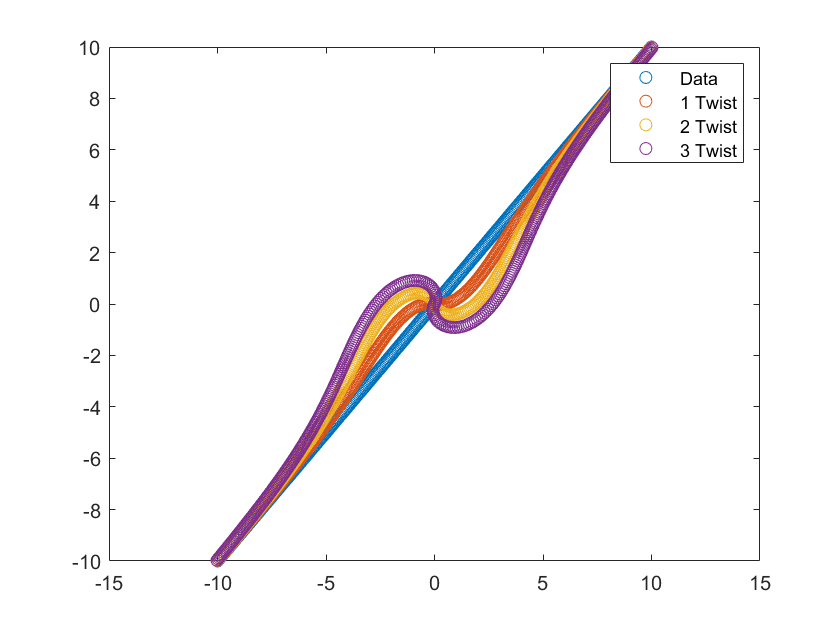
\includegraphics[scale=0.35]{SlowTwist.png}

\caption{Iterated Slow Twist of the line $y=x$.  Here, $f_1(|x|) = \exp(-\frac12 |x|^2)$, $\Theta=I$, and shown is $x, \phi(x), \phi\circ\phi(x), \phi\circ\phi\circ\phi(x)$.}
\end{figure}

\subsection{Slides}

Take an anisotropic slide function given by
\[ g(x) := \begin{bmatrix}\frac{1}{1+|x_1|^2}\\ \\ \frac12 e^{-|x_2|^2} \end{bmatrix}. \]  Figure \ref{FIG:Slide} shows iterated slides acting on two lines based on this function.

\begin{figure}[h!]
    \centering
    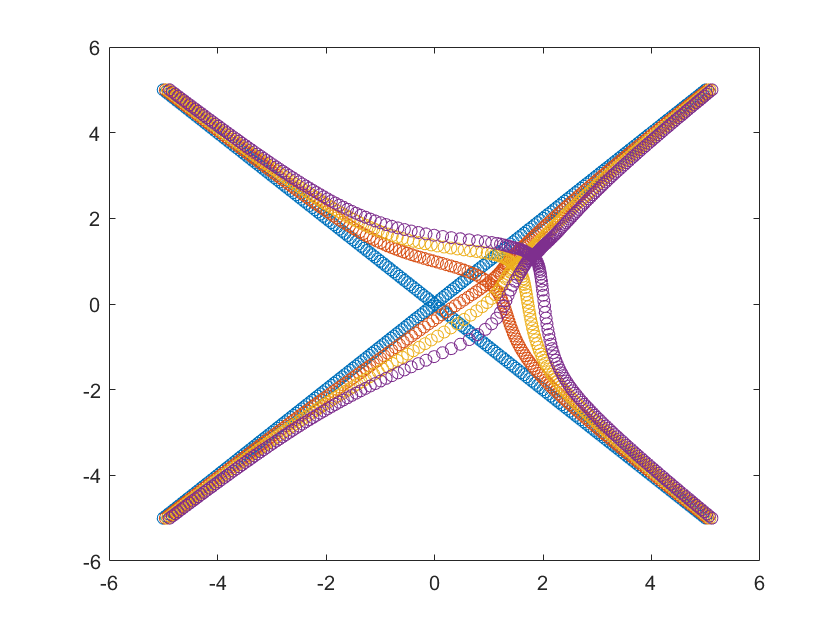
\includegraphics[scale=0.35]{Slide.png}
    \caption{Lines $y=x$ and $y=-x$ along with $\Phi(x)$, $\Phi\circ\Phi(x)$ and $\Phi\circ\Phi\circ\Phi(x)$ for $g$.}
    \label{FIG:Slide}
\end{figure}

\subsection{Motions}

You should be able to click on the pdf and these will move.

\begin{figure}[h!]
    \centering
    \animategraphics[loop,autoplay,scale=0.3]{1}{CircleSlide_}{0}{15}
    \caption{Circle undergoing a Slide.}
\end{figure}

\begin{figure}[h!]
    \centering
    \animategraphics[loop,autoplay,scale=0.3]{1}{Twist_}{0}{15}
    \caption{Line undergoing a Slow Twist.}
\end{figure}

\begin{figure}[h!]
    \centering
    \animategraphics[loop,autoplay,scale=0.3]{1}{CircleTwist_}{0}{15}
    \caption{Circle undergoing a Slow Twist.}
\end{figure}

\newpage

\section{Search Space}

If we are considering surface classification, the problem is as follows.
\begin{problem}[Shape Matching Problem]
Suppose we are given 
\begin{itemize}
\item A class of admissible transformations $\mathcal{F}$ (functions from $\R^3\to\R^3$),
\item Classes of surfaces $\{\mathcal{C}_i\}_{i=1}^N$, with surfaces represented as triangulations $(V,E,T)$, and
\item A notion of discrete distance between triangulated surfaces; e.g. a metric $d(\cdot,\cdot)$.
\end{itemize}
Solve 
\begin{equation}\label{EQ:Min}
\underset{i=1,\dots,N}\min\;\underset{f_i\in\mathcal{F}}\inf \;\textnormal{dist}(f_i(S),\mathcal{C}_i)
\end{equation}
\end{problem}

Letting $\eps>0$ be fixed, then one could compare surfaces by using the set $\mathcal{F}$ of all possible $\eps$--distortions.  Of course given the definitions above, this space is enormous by any measurement.  One might attempt to restrict to only slow twists, slides, and compositions of them; even this space is still enormous.  Thus one could restrict the choices of $\{f_i\}$ and $g$ in the definitions of slow twists and slides.  With Yifan our restriction is to a single composition Slide$\circ$Twist, and that $f_i$ should be of the form
\[ f_i(t) = e^{-\sigma_i|t|^2}, \]
and similarly for the slide
\[g(x) = \begin{bmatrix} e^{-\mu_1|x_1|^2}\\ e^{-\mu_2|x_2|^2}\\ e^{-\mu_3|x_3|^2}\\  \end{bmatrix},\]
with $\sigma_i,\mu_i\geq0$.  We also used the quaternion representation of $SO(3)$ matrices which requires three additional parameters.

Note: our restriction is arbitrary to get something to run for an experiment; we don't claim it's the right thing to do in the long run.  In principle, one should use these maps locally to compare triangulations, but this is a harder problem and we aren't sure how to do it at present.



\end{document}
